% Copyright 2004 by Till Tantau <tantau@users.sourceforge.net>.
%
% In principle, this file can be redistributed and/or modified under
% the terms of the GNU Public License, version 2.
%
% However, this file is supposed to be a template to be modified
% for your own needs. For this reason, if you use this file as a
% template and not specifically distribute it as part of a another
% package/program, I grant the extra permission to freely copy and
% modify this file as you see fit and even to delete this copyright
% notice. 

\documentclass[aspectratio=169]{beamer}
%\documentclass{beamer}

\setbeamersize{text margin left=5mm, text margin right=5mm}


\defbeamertemplate{headline}{my header}{%
\vskip1pt%
\makebox[0pt][l]{\,\insertshortauthor}%
\hspace*{\fill}\insertshorttitle/\insertshortsubtitle\hspace*{\fill}%
\llap{\insertpagenumber/\insertpresentationendpage\,}
}
\setbeamertemplate{headline}[my header]

\let\olditem\item
\renewcommand{\item}{\setlength{\itemsep}{\fill}\olditem}

\usepackage{soul}
\usepackage{tkz-euclide}
\usetikzlibrary{calc}
\usepackage[]{algorithm2e}
\usepackage{changepage}
\usepackage{amssymb}
\usepackage{xcolor}
\usepackage{mathtools}
\usepackage{tcolorbox}
\usepackage{tikz}
\usepackage{tikz-3dplot}
\usepackage[export]{adjustbox}
\usepackage{tabu}

% \usepackage[math]{cellspace}
% \cellspacetoplimit 4pt
% \cellspacebottomlimit 4pt
%\usetikzlibrary{arrows.meta}

%\setbeamertemplate{itemize items}{-}

%\usepackage{helvet}
\usefonttheme{professionalfonts} % using non standard fonts for beamer
%\usefonttheme{serif} % default family is serif
%\usepackage{fontspec}
%\setmainfont{Liberation Serif}

% There are many different themes available for Beamer. A comprehensive
% list with examples is given here:
% http://deic.uab.es/~iblanes/beamer_gallery/index_by_theme.html
% You can uncomment the themes below if you would like to use a different
% one:
%\usetheme{AnnArbor}
%\usetheme{Antibes}
%\usetheme{Bergen}
%\usetheme{Berkeley}
%\usetheme{Berlin}
%\usetheme{Boadilla}
%\usetheme{boxes}
%\usetheme{CambridgeUS}
%\usetheme{Copenhagen}
%\usetheme{Darmstadt}
%\usetheme{default}
%\usetheme{Frankfurt}
%\usetheme{Goettingen}
%\usetheme{Hannover}
%\usetheme{Ilmenau}
%\usetheme{JuanLesPins}
%\usetheme{Luebeck}
%\usetheme{Madrid}
%\usetheme{Malmoe}
%\usetheme{Marburg}
%\usetheme{Montpellier}
%\usetheme{PaloAlto}
%\usetheme{Pittsburgh}
%\usetheme{Rochester}
%\usetheme{Singapore}
%\usetheme{Szeged}
%\usetheme{Warsaw}


\def\mf{\ensuremath\mathbf}
\def\mb{\ensuremath\mathbb}
\def\mc{\ensuremath\mathcal}
\def\lp{\ensuremath\left(}
\def\rp{\ensuremath\right)}
\def\lv{\ensuremath\left\lvert}
\def\rv{\ensuremath\right\rvert}
\def\lV{\ensuremath\left\lVert}
\def\rV{\ensuremath\right\rVert}
\def\lc{\ensuremath\left\{}
\def\rc{\ensuremath\right\}}
\def\ls{\ensuremath\left[}
\def\rs{\ensuremath\right]}
\def\bmx{\ensuremath\begin{bmatrix*}[r]}
\def\emx{\ensuremath\end{bmatrix*}}
\def\bmxc{\ensuremath\begin{bmatrix*}[c]}
\def\t{\lp t\rp}
\def\k{\ls k\rs}


\newcommand{\demoex}[2]{\onslide<#1->\begin{color}{black!60} #2 \end{color}}
\newcommand{\demoexc}[3]{\onslide<#1->\begin{color}{#2} #3 \end{color}}
\newcommand{\anim}[3]{\onslide<#1->{\begin{color}{#2!60} #3 \end{color}}}
\newcommand{\ct}[1]{\lp #1\rp}
\newcommand{\dt}[1]{\ls #1\rs}
\newcommand{\cols}[2]{\begin{columns}[#1] #2 \end{columns}}
\newcommand{\col}[2]{\begin{column}{#1} #2 \end{column}}

\newcommand{\xdownarrow}[1]{%
  {\left\downarrow\vbox to #1{}\right.\kern-\nulldelimiterspace}
}

\title{Introduction to Digital Signal Processing}

% A subtitle is optional and this may be deleted
\subtitle{Fourier Representation of Discrete-Time Signals}

\author{Sivakumar Balasubramanian}
% - Give the names in the same order as the appear in the paper.
% - Use the \inst{?} command only if the authors have different
%   affiliation.

\institute[Christian Medical College] % (optional, but mostly needed)
{
  \inst{}%
  Department of Bioengineering\\
  Christian Medical College, Bagayam\\
  Vellore 632002
}
% - Use the \inst command only if there are several affiliations.
% - Keep it simple, no one is interested in your street address.

\date{}
% - Either use conference name or its abbreviation.
% - Not really informative to the audience, more for people (including
%   yourself) who are reading the slides online

\subject{Lecture slides on Introduction to DSP}
% This is only inserted into the PDF information catalog. Can be left
% out. 

% If you have a file called "university-logo-filename.xxx", where xxx
% is a graphic format that can be processed by latex or pdflatex,
% resp., then you can add a logo as follows:

% \pgfdeclareimage[height=0.5cm]{university-logo}{university-logo-filename}
% \logo{\pgfuseimage{university-logo}}

% Delete this, if you do not want the table of contents to pop up at
% the beginning of each subsection:
\AtBeginSubsection[]
{
  \begin{frame}<beamer>{Outline}
    \tableofcontents[currentsection,currentsubsection]
  \end{frame}
}

% Let's get started
\begin{document}

\begin{frame}
  \titlepage
\end{frame}


\begin{frame}[t]{Discrete-Time Fourier Series}
\begin{itemize}
  \item Continuous-time complex sinusoids have frequencies $\omega \in \lp -\infty, \infty \rp$.

  \item Discrete-time sinusoids have frequencies $\Omega \in \left( -\pi, \pi\right]$

  \item A discrete-time periodic signal $x\ls n \rs$ with fundamental period $N$ can be represented as a sum of discrete-time sinusoids,

  \[ x[n] = \sum_{k=0}^{N-1} c_k e^{j \frac{2\pi k}{N}n} \]

  \item Appropriate choice of $c_k$ will let us represent $x[n]$ as a linear combination of $e^{\frac{j2\pi k}{N}n}$.

  \item The Fourier coefficient $c_k$ can be determined by,

  \[ c_k = \frac{1}{N} \sum_{n=0}^{N-1} x[n] e^{-j\frac{2 \pi k}{N} n} \]
\end{itemize}
\end{frame}


\begin{frame}[t]{Discrete-Time Fourier Series}
\begin{itemize}
  \item $c_k$ is discrete like in the case of continuous-time Fourier series, and it is also periodic with fundamental period $N$, i.e. $c_k = c_{k + N}$.
  \begin{figure}
  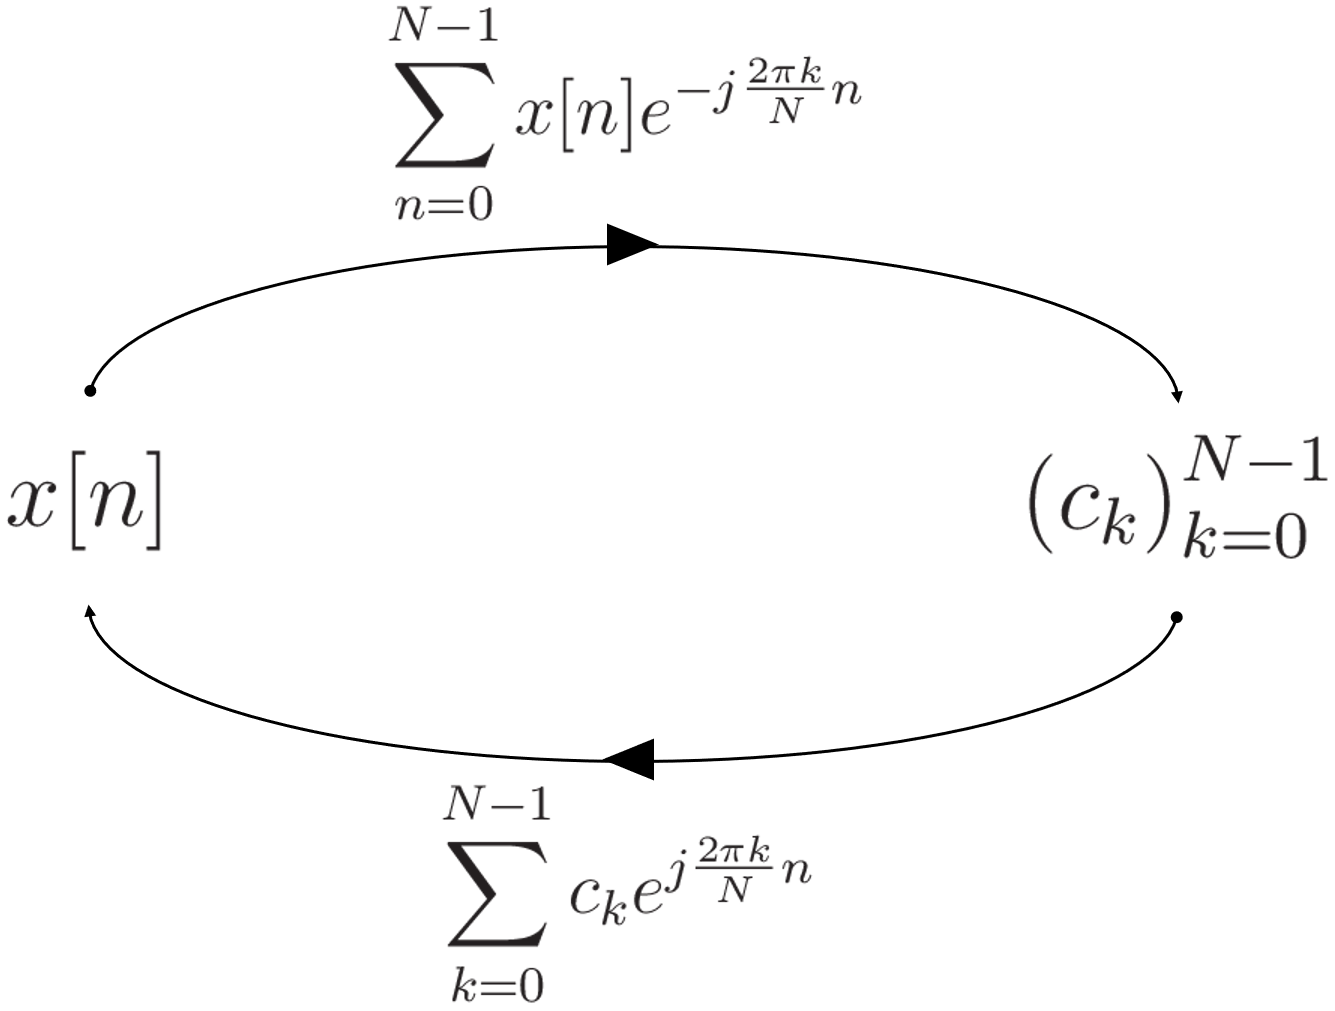
\includegraphics[width=0.55\textwidth]{img/dtfs.png}
  \end{figure}
\end{itemize}
\end{frame}


\begin{frame}[t]{Properties of Discrete-Time Fourier Series}
\begin{itemize}
  \item Fourier representation is discrete and periodic. ($c_k$ is period with fundamental period $N$)
  \item When $N = 2M$ is even, $0 < M \in \mb{Z}$.
  \[ c_{M + l} = c_{-M + l}, \quad 0 \leq l < \frac{N}{2} \]
  \item When $N = 2M + 1$ is odd, $0 < M \in \mb{Z}$.
  \[ c_{M + l} = c_{-M + l}, \quad 0 \leq l < \frac{N - 1}{2} \]
  \item Parseval's identity.
  \[ \frac{1}{N}\sum_{n=0}^{N-1} \vert x[n] \vert^2 = \sum_{k=0}^{N-1} \vert c_k \vert^2 \]
  The distribution of $\vert c_k \vert^2$ as a function of $0 \leq k < N$ is the \textit{power spectral density} of the periodic signal $x[n]$.
\end{itemize}
\end{frame}


\begin{frame}[t]{Discrete-Time Fourier Series}
Find the DTFS of  $x[n] = \begin{cases} 1, & 0 \leq n < M \\ 0, & M \leq n < N-1 \end{cases}$ with fundamental period $N$.
\end{frame}


\begin{frame}[t]{Discrete-time Fourier Transform}
\begin{itemize}
  \item Similar to the continus-time case, the Fourier representation of discrete -time aperiodic signals can be obtained as the limiting case of the a periodic signals with increasing period $N$.

  \item The discrete-time Fourier transform (DTFT) of an aperiodic signal $x[n]$ with finie energy is given by,
  \[ X\lp \Omega \rp = \sum_{n = -\infty}^{\infty} x[n] e^{-j \Omega n}, \,\,\, -\pi \leq \Omega < \pi \]

  \item $X\lp \Omega \rp$ is a continuous in $\Omega$ and periodic with period $2\pi$.

  \item Inverse DTFT,
  \[ x[n] = \frac{1}{2\pi} \int_{-\pi}^{\pi} X\lp \Omega \rp e^{j\Omega n} d\Omega \]
\end{itemize}  
\end{frame}


\begin{frame}[t]{Discrete-time Fourier Transform}
\begin{itemize}
  \item DTFT exists only if $x[n]$ is absolutely summable.
  \[ \sum_n \vert x[n] \vert < \infty  \implies \vert X\lp \Omega \rp \vert < \infty \]

  \item When $x[n]$ is only square summable, then DTFT converges to the true DTFT only in the mean squared sense.

  E.g., 
  \[ x[n] = \begin{cases} \frac{\Omega_c}{n}, & n = 0 \\ \frac{\Omega_c}{n} \frac{\sin \Omega_c n}{\Omega_c n}, & n \neq 0 \end{cases} \longrightarrow X\lp \Omega \rp  = \begin{cases} 1, & \vert \Omega \vert < \Omega_c  \\  0, & \Omega_c < \vert \Omega \vert \leq \pi \end{cases} \]
\end{itemize}  
\end{frame}


\begin{frame}[t]{Properties of DTFT}
\begin{itemize}
  \item \textbf{Linearity}: $\alpha x[n] + \beta y[n] \xleftrightarrow{\text{DTFT}} \alpha X(\Omega) + \beta Y(\Omega)$
  \item \textbf{Shift in time}: $ x[n-n_0] \xleftrightarrow{\text{DTFT}} e^{-j\Omega n_0}X(\Omega)$
  \item \textbf{Shift in frequency}: $ x[n]e^{j\Omega_0 n} \xleftrightarrow{\text{DTFT}} X(\Omega - \Omega_0) $
  \item \textbf{Symmetry in time}: $ x[n] \xleftrightarrow{\text{DTFT}} X\left(\Omega\right)$ is real.
  \item \textbf{Convolution in time}: $x[n] * y[n] \xleftrightarrow{\text{DTFT}} X(\Omega)Y(\Omega)$
  \item \textbf{Convolution in frequency}: $x[n] \cdot y[n] \xleftrightarrow{\text{DTFT}} X(\Omega) * Y(\Omega)$
\end{itemize}
\end{frame}


\begin{frame}[t]{Classification of signals based on the frequencty spectrum}
\begin{itemize}
  \item We can also classify signals based on how their energy is distributed across frequency.
  \item \textbf{Low frequency signal}. Most of the energy is concentrated around 0Hz and frequencies around 0Hz.
  \item \textbf{High frequency signal}. Very less is concentrated around 0Hz, and most of the energy is in the higher frequencies all the way upto $\omega \to \infty$.
  \item \textbf{Bandpass signal}. Very less concentration around 0Hz and at high frequencies. Most of the energy is concentrated within a band of finite frequencies. 
  \item \textbf{Bandlimited signal}. Signal energy is uniformly zero beyond a particular frequency, i.e. $\vert X\lp \omega \rp \vert = 0, \,\, \forall \vert \omega \vert > \omega_b$.
\end{itemize}
\end{frame}


\begin{frame}[t]{Bandwidth of a signal}
\begin{itemize}
  \item The band of frequencies over which most of the energy is distributed is the \textit{bandwidth} of the signal.
  \item Several ways to define the bandwidth of a signal.
  \item \textbf{3 dB bandwidth}. Frequency range over which the spectral density is above a particular threshold.

  Threshold value is often defined relative to the max. value of the spectal density.
\end{itemize}
\end{frame}


\begin{frame}[t]
  \frametitle{Frequency-Domain and Time-Domain Properties}
  \begin{itemize}
    \item \textbf{Continuous-Time, Periodic} $\longrightarrow$
    \item \textbf{Discrete-Time, Non-Periodic} $\longrightarrow$
    \item \textbf{Continuous-Frequency, Periodic} $\longrightarrow$
    \item \textbf{Discrete-Frequency, Non-Periodic} $\longrightarrow$
  \end{itemize}
\end{frame}

\end{document}